\documentclass{article} % For LaTeX2e
\usepackage{cos424,times}
\usepackage{hyperref}
\usepackage{url}
\usepackage{graphicx}
\usepackage{enumitem}
\usepackage{wrapfig}
% For LaTeX2e
\usepackage{cos424,times}
\usepackage{hyperref}
\usepackage{url}
\usepackage{graphicx}
\usepackage{wrapfig}
\usepackage{amsmath}
\usepackage{enumitem}
\usepackage{booktabs}
% packages that allow mathematical formatting
\usepackage{setspace}
% package that allows you to change spacing
\usepackage{comment}
% text become 1.5 spaced

\usepackage{fullpage}
% package that specifies normal margins
\usepackage{amsmath}
\usepackage{graphicx}
\usepackage{float}
\usepackage{listings}
\usepackage{subfig}
\usepackage{bbm}
\usepackage{multirow}
\usepackage{booktabs}

\title{CME Homework Assignment 2 Computational Work}


\author{
Jacob Perricone \\
Stanford University\\
\texttt{jacobp2@stanford.edu} \\, \and
\textbf{Ian Shaw}\\
Stanford University\\
\texttt{ieshaw@stanford.edu} \\, \and
\textbf{Weronika \`Swi\c echowicz} \\ 
Stanford University\\
\texttt{wswiecho@stanford.edu}
}




\newcommand{\fix}{\marginpar{FIX}}

\usepackage{xcolor}
%\usepackage{mathbb}
\usepackage{sympytex}
\usepackage{color}
\usepackage{sectsty}
\sectionfont{\LARGE\underline}
\subsectionfont{\underline\normalsize}
\subsubsectionfont{\underline\normalsize\itshape}


\definecolor{mygreen}{rgb}{0,0.6,0}
\definecolor{mygray}{rgb}{0.5,0.5,0.5}
\definecolor{mymauve}{rgb}{0.58,0,0.82}

\lstset{ %
backgroundcolor=\color{white},   % choose the background color; you must add \usepackage{color} or \usepackage{xcolor}
basicstyle=\footnotesize,
flexiblecolumns=true      % the size of the fonts that are used for the code
breakatwhitespace=false,         % sets if automatic breaks should only happen at whitespace
breaklines=true,                 % sets automatic line breaking
captionpos=b,                    % sets the caption-position to bottom
commentstyle=\color{mygreen},    % comment style
deletekeywords={...},            % if you want to delete keywords from the given language
    escapeinside={\%*}{*)},          % if you want to add LaTeX within your code
    extendedchars=true,              % lets you use non-ASCII characters; for 8-bits encodings only, does not work with UTF-8
    frame=single,                    % adds a frame around the code
    keepspaces=true,                 % keeps spaces in text, useful for keeping indentation of code (possibly needs columns=flexible)
    keywordstyle=\color{blue},       % keyword style
    language=Matlab,                 % the language of the code
    otherkeywords={*,...},           % if you want to add more keywords to the set
    numbers=left,                    % where to put the line-numbers; possible values are (none, left, right)
    numbersep=5pt,                   % how far the line-numbers are from the code
    numberstyle=\tiny\color{mygray}, % the style that is used for the line-numbers
    %rulecolor=\color{black},         % if not set, the frame-color may be changed on line-breaks within not-black text (e.g. comments (green here))
    showspaces=false,                % show spaces everywhere adding particular underscores; it overrides 'showstringspaces'
    showstringspaces=false,          % underline spaces within strings only
    showtabs=false,                  % show tabs within strings adding particular underscores
    stepnumber=2,                    % the step between two line-numbers. If it's 1, each line will be numbered
    stringstyle=\color{mymauve},     % string literal style
    tabsize=2,                     % sets default tabsize to 2 spaces
    title=\lstname,
    % Single frame around code                               % show the filename of files included with \lstinputlisting; also try caption instead of title
    }
    
    \newcommand{\E}{{\mbox {\bf E}}}
    \newcommand{\me}{\mathrm{e}}
    \newcommand{\I}{\mathbbm{1}}
    \newcommand{\R}{\mathbbm{R}}
    \newcommand{\Q}{\mathbbm{Q}}
    \newcommand{\Z}{\mathbb{Z}}
    \newcommand{\N}{\operatorname{N}}
    \newcommand{\C}{\operatorname{C}}
    \newcommand{\f}[1][]{\hat{#1}}
    \newcommand{\rev}[1]{\frac{1}{#1}}
    % \newcommand{+binomial}[3][2]{(#2 + #3)^#1}
    \newcommand{\prev}[1]{#1_{t-1}}
    \newcommand{\nex}[1]{#1_{t+1}}
    \newcommand{\now}[1]{#1_t}
    \newcommand{\ttwo}[1]{\now{#1}^{2}}
    \newcommand*{\dprime}{^{\prime\prime}\mkern-1.2mu}
    \newcommand*{\tprime}{^{\prime\prime\prime}\mkern-1.2mu}
    
    \newcommand{\ptwo}[1]{\prev{#1^{2}}}
    \newcommand{\h}[1]{\expandafter\hat#1}
    \newcommand{\ti}[1]{\widetilde{#1}}
    \newcommand{\B}[1]{\mathbf#1}
    \newcommand{\ii}[1]{\mathit#1}
    \newcommand{\that}[1]{\mathbf{\hat{#1}}}
    \newcommand{\ttil}[1]{\mathbf{\tilde{#1}}}
    \newcommand{\new}{\marginpar{NEW}}
    \begin{document}
    \newcommand{\argmin}{\operatornamewithlimits{argmin}}.
    \maketitle
    
    
    

\section*{(20pts) Computation Team Work: }
 Now consider the sensor localization problem on plane $R^2$ with two sensors $x_1$ and $x_2$ and three anchors $a_1=(1;0)$, $a_2=(-1;0)$ and $a_3=(0;2)$. Suppose we know the (Euclidean) distances from one sensor to $a_1$ and $a_2$, denoted by $d_{11}$ and $d_{12}$; distances of the other to $a_2$ and $a_3$, denoted by $d_{22}$ and $d_{23}$; and the distance between the two sensors, denoted by $\hat{d}_{12}$. Then, from the anchor and distance information we like locate the sensor positions $x_1, x_2\in R^2$?

Do the following numerical experimentations:
\begin{itemize}
\item Generate two sensor points anywhere and try the SOCP relaxation model
\[
\begin{array}{cl}
\|x_1-a_i\|^2 &\le d^2_{1i},\ i=1,2\\
\|x_2-a_i\|^2 &\le d^2_{1i},\ i=2,3\\
\|x_1-x_2\|^2&\le \hat{d}^2_{12}.
\end{array}
\]
Did you find the correct locations? What have you observed?

\rule{\textwidth}{1pt}
In order to examine the performance of the SOCP relaxation model for sensor localization in $\R^2$, lets examine some interesting possible cases. First, let us consider fixing the point $x_1$ in the center of the convex hull of the anchors. That is, let $x_1$ be fixed at $[0,1]$, and examine the performance of the optimization for $x_2$ points both within the convex hull and outside the hull. 



\subsection*{$x_1$ Fixed in Center of Convex Hull}
First observe that it is interesting to examine the optimization's performance in locating each of the sensors individually. 

The subplots below show the errors of the SOCP relaxation for $x_1 = \begin{bmatrix} 0 \\ 1 \end{bmatrix}$ and $x_2$ varying across the meshgrid. The first plot is the error in locating $x_1$, the second plot $x_2$ and the third plot  the total error. The blue dot indicates the fixed $x_1$ point. Recall that $x_1$ only has distance information about $a_1$ and $a_2$ whereas $x_2$ has information on $a_2, a_3$. 


\begin{figure}[H]
\centering
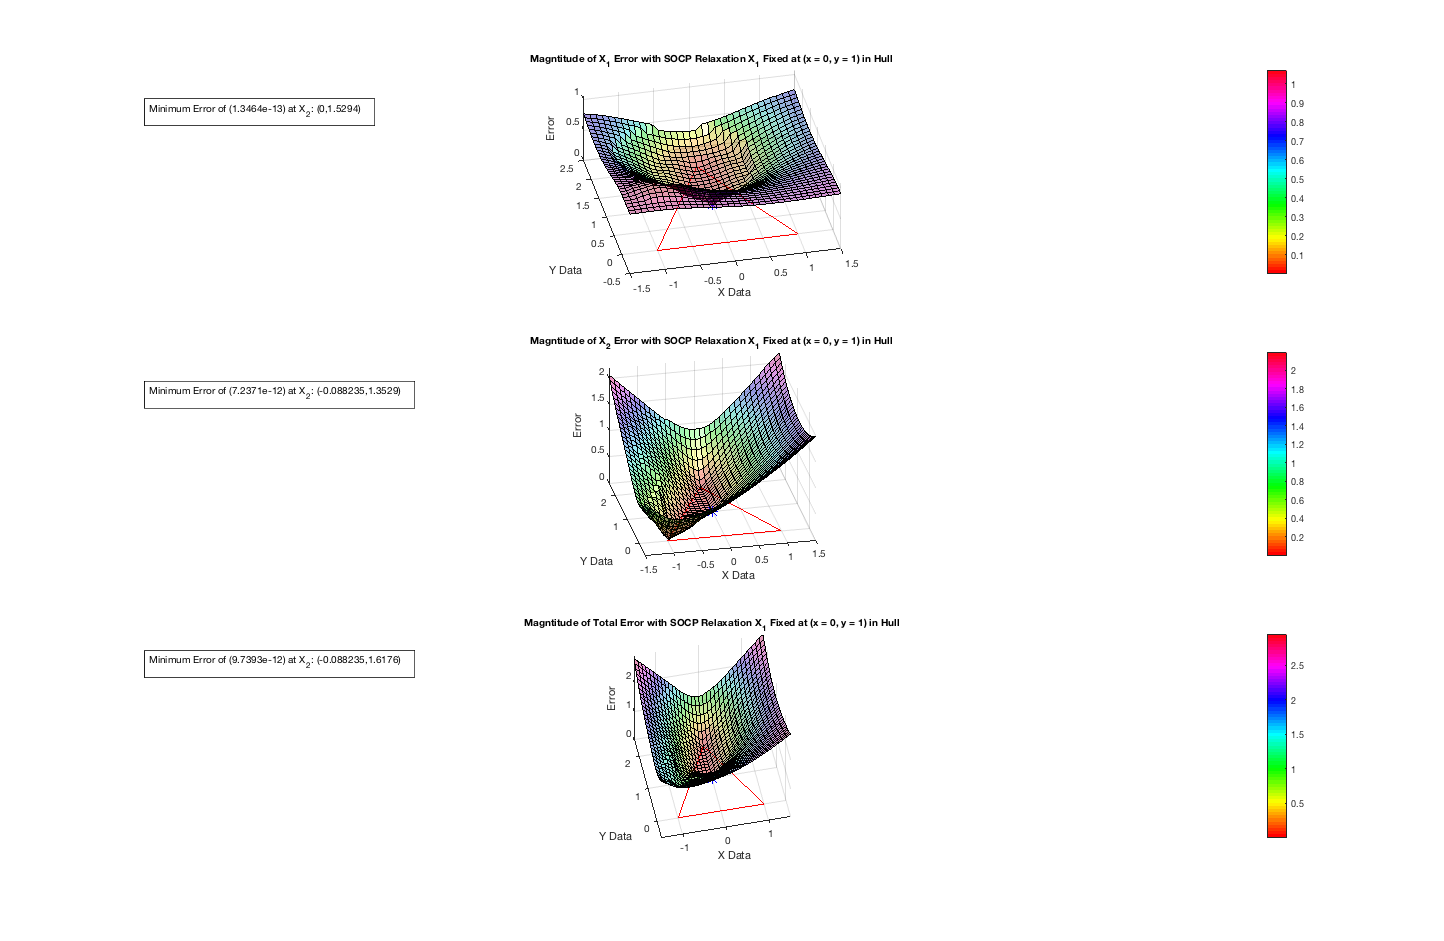
\includegraphics[width=\textwidth,height=15cm]{SOCP_Centerhull.png}
\end{figure}


Observe that the error in locating $x_1$ when $x_2$ is close to $a_3$ is very low and increases dramatically when $x_2$ is closer to $a_1$ or $a_2$, even within the convex hull. This intuitively makes sense, since when $x_2$ is close to either anchors within the hull, it in effect is very easily to locate and could be loosely thought of as acting as an additional anchor point. When $x_2$ outside the convex hull the error is uniformly large, which is expected in SOCP as per homework 1.  Now for the error in locating $x_2$, we observe an interesting result. When $x_2$ is along the vertex connecting $a_2$ to $a_3$ the optimization procedure is able to perform very well. However as $x_2$ drifts towards $a_1$ or outside the convex hull, the error increases dramatically. This is because we only have distance information for $x_2$ with $a_2,a_3$. So in effect, when $x_2$ is near $a_1$, the optimization is unable to find forces such that the total force on each anchor point is zero. 

\subsection*{$x_1$ Fixed near $a_1$}


Now let us examine the performance of the optimization when $x_1$ is fixed closed to $a_1$, $x_1 = \begin{bmatrix} .95 \\ .05 \end{bmatrix}$. 

\begin{figure}[H]
\centering
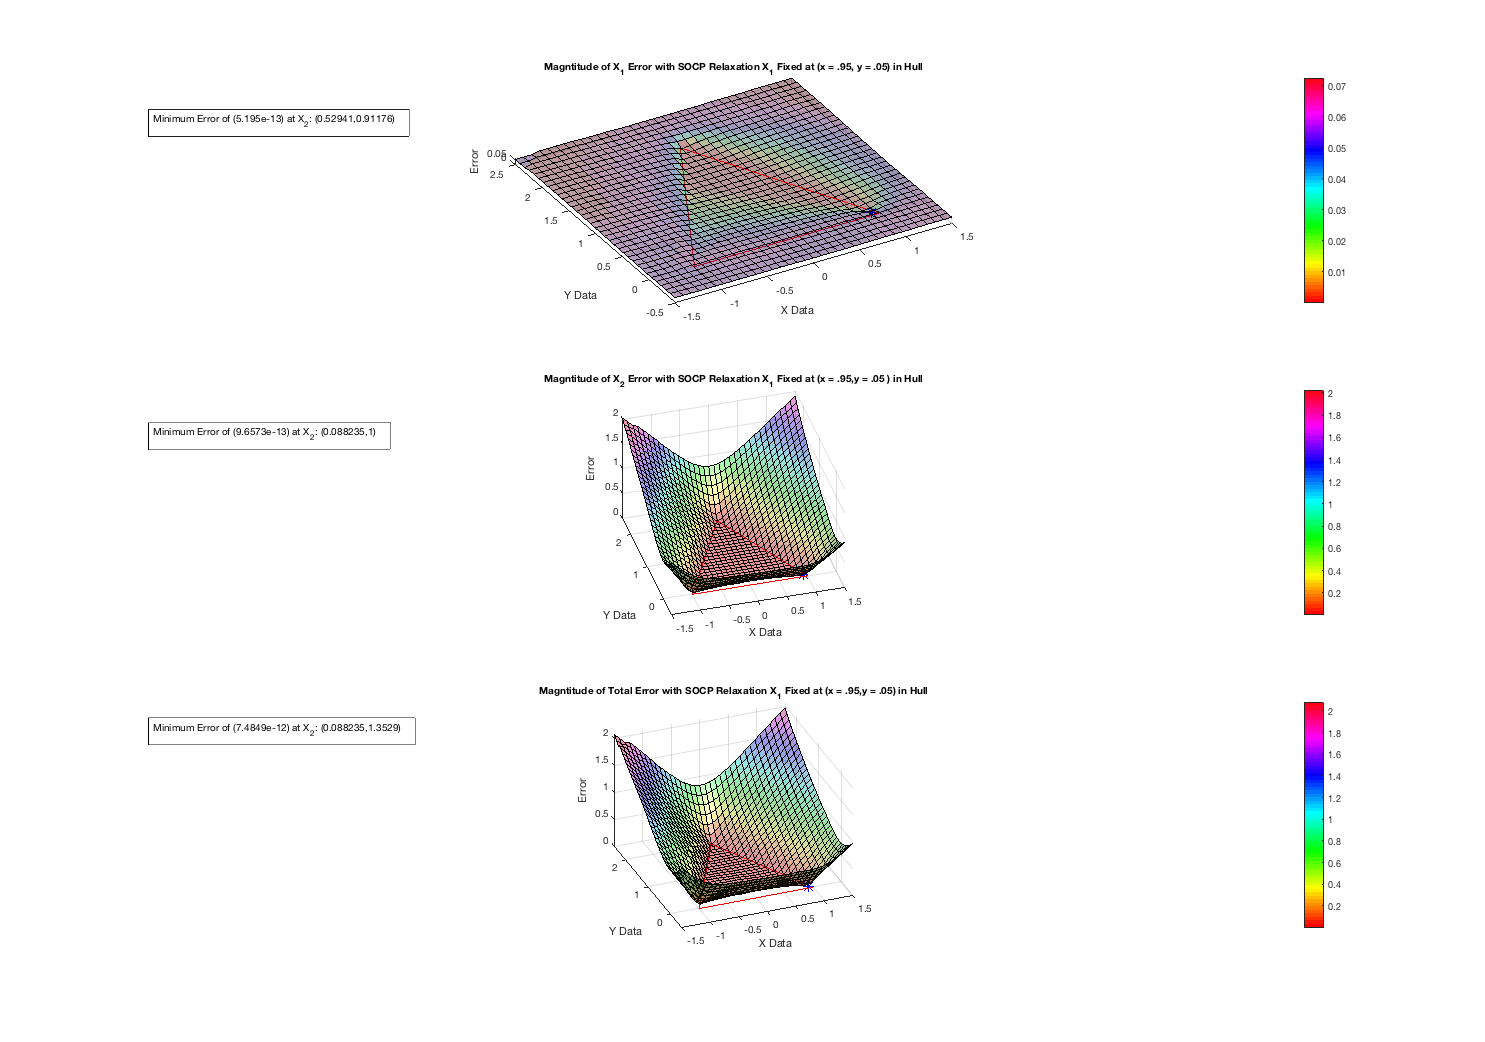
\includegraphics[width=\textwidth,height=15cm]{SOCP_NEAR_A1.png}
\end{figure}

The first thing to notice is that $x_1$ is uniformly easy to locate when $x_1$ is near the anchor point. Because of this, $x_1$ does not create an extra layer of uncertainty in the location of $x_2$, and thus the results for the SOCP relaxation in $\R^2$ with two sensors become very much similar to the problem of locating one sensor. The error is low within the convex hull and increases dramatically outside of it. This is due to the fact that when outside the convex hull, the forces acting upon the sensor points are unable to balance. 




\rule{\textwidth}{1pt}



\item Now try the SDP relaxation: find $X=[x_1,\ x_2]\in R^{2\times 2}$ and
\[Z=\left(\begin{array}{cc}
              I & X\\
              X^T& Y\end{array}\right)\in S^4
\]
to meet the constraints in the standard form:
\[\begin{array}{cl}
(1;0;0;0)(1;0;0;0)^T\bullet Z &=1,\\
(0;1;0;0)(0;1;0;0)^T\bullet Z& =1,\\
(1;1;0;0)(1;1;0;0)^T\bullet Z& =2,\\
(a_i;-1;0)(a_i;-1;0)^T\bullet Z &= d^2_{1i},\ i=1,2,\\
(a_i;0;-1)(a_i;0;-1)^T\bullet Z &= d^2_{2i},\ i=2,3,\\
(0;0;1;-1)(0;0;1;-1)^T\bullet Z&=\hat{d}^2_{12},\\
Z &\succeq 0\in S^4.
\end{array}
\]
Did you find the correct locations? What have you observed? Can you conclude something? 

\rule{\textwidth}{1pt}

\subsection*{$x_1$ Fixed in Center of Convex Hull}

Lets consider the same approach as in SDP and fix $x_1$ in the center of the Hull and close to an anchor point. The 
\begin{figure}[H]
\centering
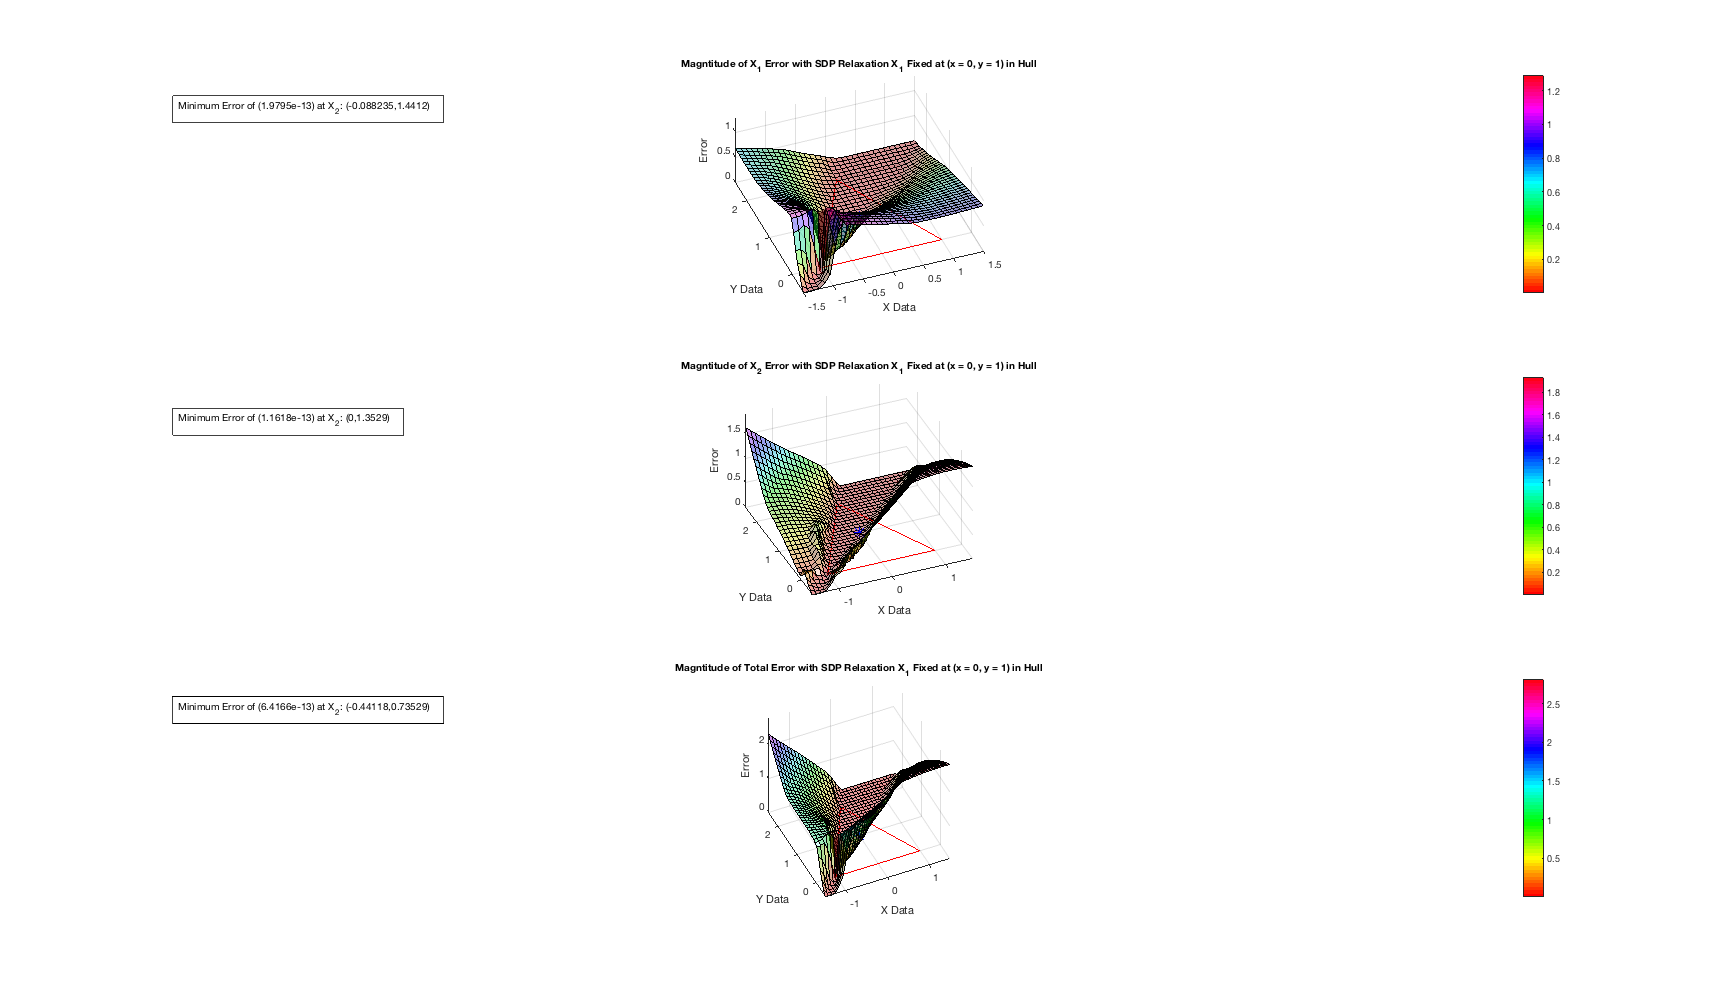
\includegraphics[width=\textwidth,height=15cm]{SDPCenter.png}
\end{figure}

Similar to SDP, when $x_1$ is placed in the center of the convex hull, the error in locating $x_1$ decreases as $x_2$ approaches the vertex $a_2,a_3$, with the optimum $x_2$ point being very close to $x_2$ . The error increases when $x_2$ drifts outside the convex Hull, but not as dramatically as with SOCP relaxation. The error in $x_2$ similarly increases as $x_2$ drifts away from the vertex connecting $a_2$ and $a_3$. This is because the stress matrix in the SOCP relaxation is not of full rank. When the SDP has a unique solution along the vertex, the results are good, however, when $x_2$ drifts away from the vertex $a_2 \rightarrow a_3$, the U is rank deficient. 

\subsection*{$x_1$ Fixed near $a_1$}


\begin{figure}[H]
\centering
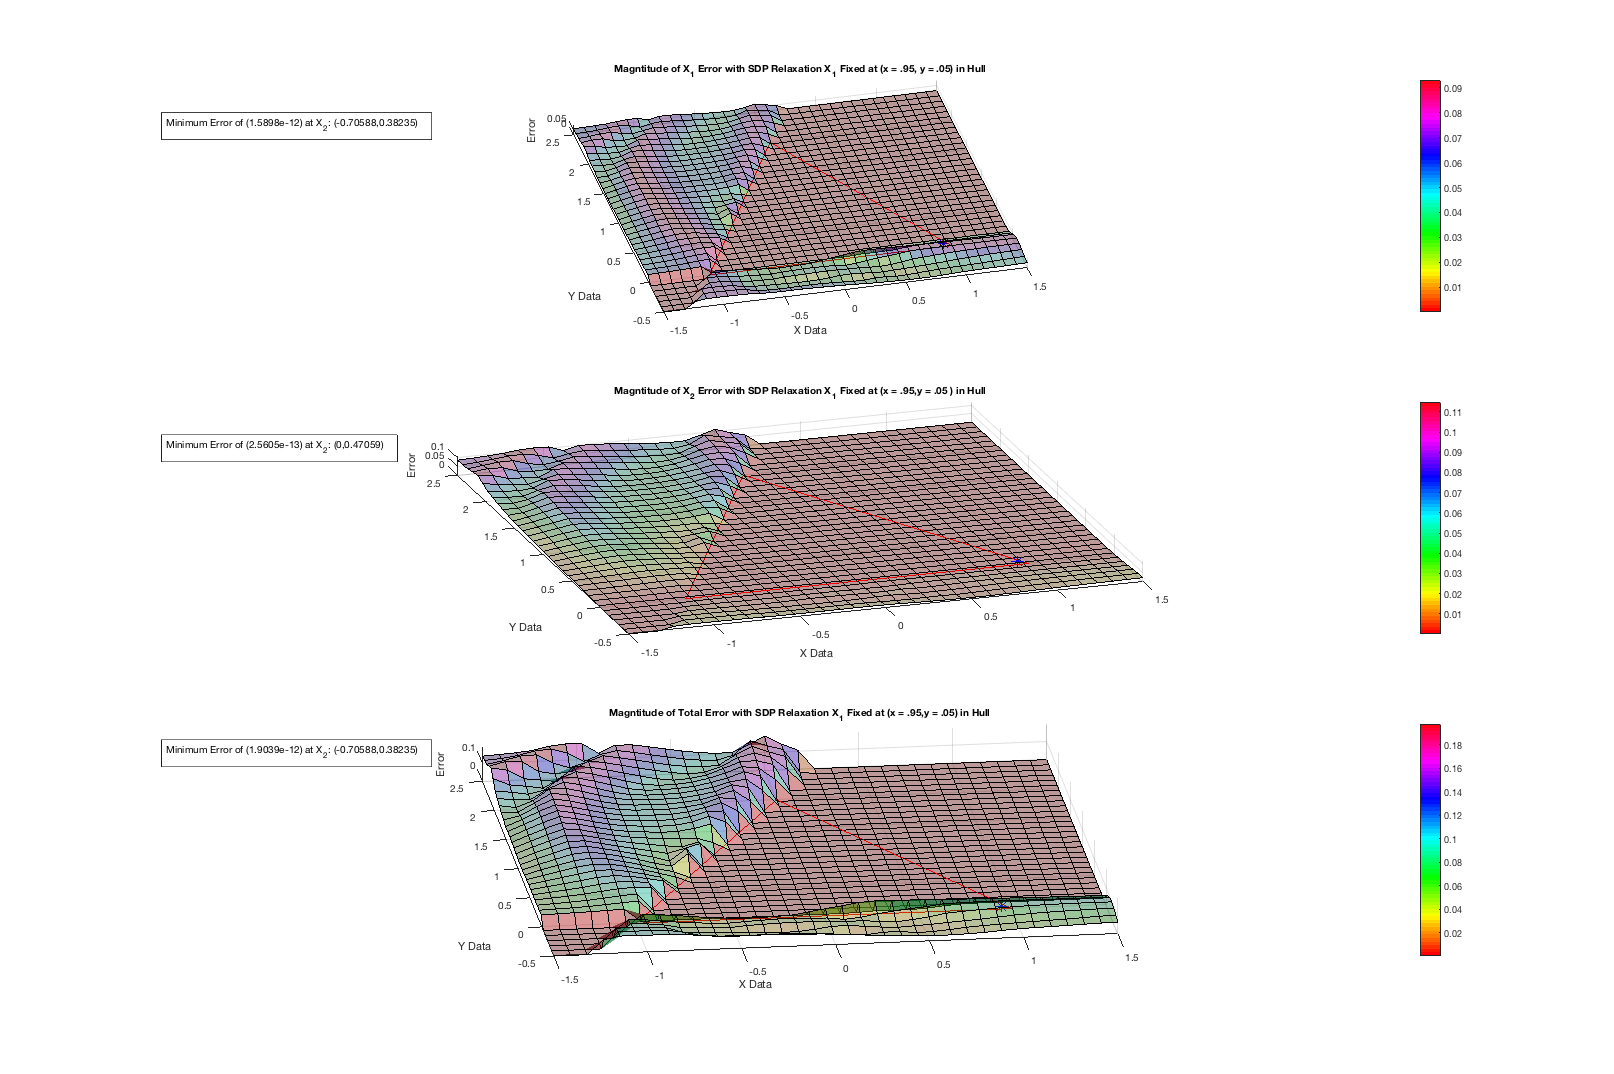
\includegraphics[width=\textwidth,height=15cm]{SDPNEAR1.png}
\end{figure}

Now when $x_1$ is fixed near $a_1$, the solution is pretty good (both for $x_2$ and $x_1$) for $x_2$ points both in and outside of the convex hull. The error increases slightly as $x_2$ leaves the convex Hull, but not dramatically. Overall, though, the results for SDP when $x_1$ is close to $a_1$ are greatly superior to that of SOCP. Intuitively, the SDP relaxation allows for the internal forces to have two directions where SOCP only allows for one. When the stress matrix has full rank, the SDP relaxation has a larger possibility to balance the force in that position and can thus perform better. Howevever, when the dual stress matrix in SDP does not have full rank, the points are not localizable. 



\begin{lstlisting}
clear all
close all


a = [1, -1, 0; 0, 0, 2];


x1 = [2*rand(25,1) + -1, 2*rand(25,1)];
x2 = [2*rand(25,1) + -1, 2*rand(25,1)];


dist_x1 = pdist2(x1, a(:,1:2)');
dist_x2 = pdist2(x2, a(:,2:3)');
dhat = pdist2(x1, x2);



%% Fix point in convex hull



%% Middle of HULL

clear all
close all


a = [1, -1, 0; 0, 0, 2];
%%

[X_1, Y_1] = meshgrid(linspace(-1.5, 1.5,35)',linspace(-.5,2.5,35)');

Cx1_error_SOCP = zeros(size(X_1,1), size(Y_1,1));
Cx2_error_SOCP = zeros(size(X_1,1), size(Y_1,1));
Ctotal_error_SOCP = zeros(size(X_1,1), size(Y_1,1));


Vx1_error_SOCP = zeros(size(X_1,1), size(Y_1,1));
Vx2_error_SOCP = zeros(size(X_1,1), size(Y_1,1));
Vtotal_error_SOCP = zeros(size(X_1,1), size(Y_1,1));



for j=1:size(X_1, 1)
    j;
    for l=1:size(Y_1,1)
        l;
        x1_center = [0,1];
        dist_x1_center = pdist2(x1_center, a(:,1:2)');
        
        x1_vertex = [.95,.05];
        dist_x1_vertex = pdist2(x1_vertex, a(:,1:2)');
        
        x2 = [X_1(j,l),Y_1(j,l)];
        dist_x2 = pdist2(x2, a(:,2:3)');
        
        dhat_center = pdist2(x1_center, x2);
        dhat_vertex = pdist2(x1_vertex, x2);
        
        cvx_begin quiet
            variables x_1(2) x_2(2)
            minimize 0
            subject to
            for i = 1:2
                norm(x_1 - a(:, i),2) <= dist_x1_center(i);
                norm(x_2 - a(:,i+1),2) <= dist_x2(i);
                norm(x_1 - x_2,2) <= dhat_center;
            end
        cvx_end
        
        Cx1_error_SOCP(j,l) = norm(x_1 - x1_center');
        Cx2_error_SOCP(j,l) = norm(x_2 - x2');
        Ctotal_error_SOCP(j,l) = Cx1_error_SOCP(j,l) +  Cx2_error_SOCP(j,l);
        Cdistance(j,l) = dhat_center;
        
        cvx_begin quiet
            variables x_1(2) x_2(2)
            minimize 0
            subject to
            for i = 1:2
                norm(x_1 - a(:, i),2) <= dist_x1_vertex(i);
                norm(x_2 - a(:,i+1),2) <= dist_x2(i);
                norm(x_1 - x_2,2) <= dhat_vertex;
            end
        cvx_end
        
        Vx1_error_SOCP(j,l) = norm(x_1 - x1_vertex');
        Vx2_error_SOCP(j,l) = norm(x_2 - x2');
        Vtotal_error_SOCP(j,l) = Vx1_error_SOCP(j,l) +  Vx2_error_SOCP(j,l);
        Vdistance(j,l) = dhat_vertex;
        
        
    end
end
 
%%
figure()
subplot(3,1,1)
surf(X_1, Y_1, Cx1_error_SOCP)
colormap hsv
alpha(.4)
colorbar
view(-30,30); camlight; axis image



title('Magntitude of X_1 Error with SOCP Relaxation X_1 Fixed at (x = 0, y = 1) in Hull', 'FontSize', 10)
xlabel('X Data')
ylabel('Y Data')
zlabel('Error')
[mx,k] = min(Cx1_error_SOCP(:));
[ix,jx] = ind2sub(size(Cx1_error_SOCP),k);
dim = [.10 .595 .3 .3];
str = strcat('Minimum Error of (', num2str(Cx1_error_SOCP(ix,jx)),')', ' at X_2: (', num2str(X_1(ix,jx)), ',', num2str(Y_1(ix,jx)),')');
annotation('textbox',dim,'String',str,'FitBoxToText','on', 'FontSize',10);

hold on
tmp = a;
tmp(:,4) = tmp(:,1);
plot3(tmp(1,:), tmp(2,:), zeros(size(tmp(2,:))), '-r')
plot3(x1_center(1), x1_center(2), 0, '-*b','MarkerSize',10)
xlabel('X Data')
ylabel('Y Data')
hold off


subplot(3,1,2)
surf(X_1, Y_1, Cx2_error_SOCP)
colormap hsv
alpha(.4)
colorbar
view(-30,30); camlight; axis image


title('Magntitude of X_2 Error with SOCP Relaxation X_1 Fixed at (x = 0, y = 1) in Hull', 'FontSize', 10)
xlabel('X Data')
ylabel('Y Data')
zlabel('Error')

[mx,k] = min(Cx2_error_SOCP(:));
[ix,jx] = ind2sub(size(Cx2_error_SOCP),k);
dim = [.10 .295 .3 .3];
str = strcat('Minimum Error of (', num2str(Cx2_error_SOCP(ix,jx)),')', ' at X_2: (', num2str(X_1(ix,jx)), ',', num2str(Y_1(ix,jx)),')');
annotation('textbox',dim,'String',str,'FitBoxToText','on', 'FontSize',10);

hold on
tmp = a;
tmp(:,4) = tmp(:,1);
plot3(tmp(1,:), tmp(2,:), zeros(size(tmp(2,:))), '-r')
plot3(x1_center(1), x1_center(2), 0, '-*b','MarkerSize',10)
xlabel('X Data')
ylabel('Y Data')
hold off


subplot(3,1,3)
surf(X_1, Y_1, Ctotal_error_SOCP)
colormap hsv
alpha(.4)
colorbar
view(-30,30); camlight; axis image



title('Magntitude of Total Error with SOCP Relaxation X_1 Fixed at (x = 0, y = 1) in Hull', 'FontSize', 10)
xlabel('X Data')
ylabel('Y Data')
zlabel('Error')

[mx,k] = min(Ctotal_error_SOCP(:));
[ix,jx] = ind2sub(size(Ctotal_error_SOCP),k);
dim = [.10 .009 .3 .3];
str = strcat('Minimum Error of (', num2str(Ctotal_error_SOCP(ix,jx)),')', ' at X_2: (', num2str(X_1(ix,jx)), ',', num2str(Y_1(ix,jx)),')');
annotation('textbox',dim,'String',str,'FitBoxToText','on', 'FontSize',10);

hold on
tmp = a;
tmp(:,4) = tmp(:,1);
plot3(tmp(1,:), tmp(2,:), zeros(size(tmp(2,:))), '-r')
plot3(x1_center(1), x1_center(2), 0, '-*b','MarkerSize',10)
xlabel('X Data')
ylabel('Y Data')
hold off


%
figure()
subplot(3,1,1)
surf(X_1, Y_1, Vx1_error_SOCP)
colormap hsv
alpha(.4)
colorbar
view(-30,30); camlight; axis image




title('Magntitude of X_1 Error with SOCP Relaxation X_1 Fixed at (x = .95, y = .05) in Hull', 'FontSize', 10)
xlabel('X Data')
ylabel('Y Data')
zlabel('Error')



[mx,k] = min(Vx1_error_SOCP(:));
[ix,jx] = ind2sub(size(Vx1_error_SOCP),k);
dim = [.10 .595 .3 .3];
str = strcat('Minimum Error of (', num2str(Vx1_error_SOCP(ix,jx)),')', ' at X_2: (', num2str(X_1(ix,jx)), ',', num2str(Y_1(ix,jx)),')');
annotation('textbox',dim,'String',str,'FitBoxToText','on', 'FontSize',10);

hold on
tmp = a;
tmp(:,4) = tmp(:,1);
plot3(tmp(1,:), tmp(2,:), zeros(size(tmp(2,:))), '-r')
plot3(x1_vertex(1), x1_vertex(2), 0, '-*b','MarkerSize',10)
xlabel('X Data')
ylabel('Y Data')
hold off


subplot(3,1,2)


surf(X_1, Y_1, Vx2_error_SOCP)
colormap hsv
alpha(.4)
colorbar
view(-30,30); camlight; axis image


title('Magntitude of X_2 Error with SOCP Relaxation X_1 Fixed at (x = .95,y = .05 ) in Hull', 'FontSize', 10)
xlabel('X Data')
ylabel('Y Data')
zlabel('Error')
[mx,k] = min(Vx2_error_SOCP(:));
[ix,jx] = ind2sub(size(Vx2_error_SOCP),k);
dim = [.10 .295 .3 .3];
str = strcat('Minimum Error of (', num2str(Vx2_error_SOCP(ix,jx)),')', ' at X_2: (', num2str(X_1(ix,jx)), ',', num2str(Y_1(ix,jx)),')');
annotation('textbox',dim,'String',str,'FitBoxToText','on', 'FontSize',10);

hold on
tmp = a;
tmp(:,4) = tmp(:,1);
plot3(tmp(1,:), tmp(2,:), zeros(size(tmp(2,:))), '-r')
plot3(x1_vertex(1), x1_vertex(2), 0, '-*b','MarkerSize',10)
xlabel('X Data')
ylabel('Y Data')
hold off


subplot(3,1,3)
surf(X_1, Y_1, Vtotal_error_SOCP)
colormap hsv
alpha(.4)
colorbar
view(-30,30); camlight; axis image


title('Magntitude of Total Error with SOCP Relaxation X_1 Fixed at (x = .95,y = .05) in Hull', 'FontSize', 10)
xlabel('X Data')
ylabel('Y Data')
zlabel('Error')
[mx,k] = min(Vtotal_error_SOCP(:));
[ix,jx] = ind2sub(size(Vtotal_error_SOCP),k);
dim = [.1 .011 .3 .3];
str = strcat('Minimum Error of (', num2str(Vtotal_error_SOCP(ix,jx)),')', ' at X_2: (', num2str(X_1(ix,jx)), ',', num2str(Y_1(ix,jx)),')');
annotation('textbox',dim,'String',str,'FitBoxToText','on', 'FontSize',10);


hold on
tmp = a;
tmp(:,4) = tmp(:,1);
plot3(tmp(1,:), tmp(2,:), zeros(size(tmp(2,:))), '-r')
plot3(x1_vertex(1), x1_vertex(2), 0, '-*b','MarkerSize',10)
xlabel('X Data')
ylabel('Y Data')
hold off


%%

clear all

a = [1, -1, 0; 0, 0, 2];



%
[X_1, Y_1] = meshgrid(linspace(-1.5, 1.5,35)',linspace(-.5,2.5,35)');

Cx1_error_SDP = zeros(size(X_1,1), size(Y_1,1));
Cx2_error_SDP = zeros(size(X_1,1), size(Y_1,1));
Ctotal_error_SDP = zeros(size(X_1,1), size(Y_1,1));


Vx1_error_SDP = zeros(size(X_1,1), size(Y_1,1));
Vx2_error_SDP = zeros(size(X_1,1), size(Y_1,1));
Vtotal_error_SDP = zeros(size(X_1,1), size(Y_1,1));

A1 = [1; 0; 0; 0];   A2 = [0; 1; 0; 0];   A3 = [1; 1; 0; 0];
A = [A1, A2, A3];
a = [1, -1, 0; 0, 0, 2];
for j=1:size(X_1, 1)
    j;
    for l=1:size(Y_1,1)
        
        x1_center = [0,1];
        dist_x1_center = pdist2(x1_center, a(:,1:2)');
        
        x1_vertex = [.95,.05];
        dist_x1_vertex = pdist2(x1_vertex, a(:,1:2)');
        
        x2 = [X_1(j,l),Y_1(j,l)];
        dist_x2 = pdist2(x2, a(:,2:3)');
        
        dhat_center = pdist2(x1_center, x2);
        dhat_vertex = pdist2(x1_vertex, x2);
        
        cvx_begin sdp quiet
            variable Z(4,4) symmetric
            minimize(0);
            subject to

            sum(dot(A(:,1)*A(:,1)', Z)) == 1;
            sum(dot(A(:,2)*A(:,2)', Z)) == 1;
            sum(dot(A(:,3)*A(:,3)', Z)) == 2;
            
            for i = 1:2
                
                sum(dot([a(:, i); -1; 0] * [a(:, i); -1; 0]',  Z))...
                    == dist_x1_center(i)^2;
                sum(dot([a(:, i+1); 0;  -1] * [a(:, i+1); 0; -1]', Z))...
                    == dist_x2(i)^2;
            end

            sum(dot([0; 0; 1; -1] * [0; 0; 1; -1]', Z)) == dhat_center^2 ;

            Z >= 0;

        cvx_end
        
        x_1 = [Z(3,1), Z(3,2)]';
        x_2 = [Z(4,1), Z(4,2)]';

        
        
            
        Cx1_error_SDP(j,l) = norm(x_1 - x1_center');
        Cx2_error_SDP(j,l) = norm(x_2 - x2');
        Ctotal_error_SDP(j,l) = Cx1_error_SDP(j,l) +  Cx2_error_SDP(j,l);
        Cdistance(j,l) = dhat_center;
        

        cvx_begin sdp quiet
            variable Z(4,4) symmetric
            minimize(0);
            subject to

            sum(dot(A(:,1)*A(:,1)', Z)) == 1;
            sum(dot(A(:,2)*A(:,2)', Z)) == 1;
            sum(dot(A(:,3)*A(:,3)', Z)) == 2;

            for i = 1:2
                sum(dot([a(:, i); -1; 0] * [a(:, i); -1; 0]',  Z))...
                    == dist_x1_vertex(i)^2;
                sum(dot([a(:, i+1); 0;  -1] * [a(:, i+1); 0; -1]', Z))...
                    == dist_x2(i)^2;
            end

            sum(dot([0; 0; 1; -1] * [0; 0; 1; -1]', Z)) == dhat_vertex^2 ;

            Z >= 0;

        cvx_end
        
        
        x_1 = [Z(3,1), Z(3,2)]';
        x_2 = [Z(4,1), Z(4,2)]';
        

        
        if isnan(x_1(1)) || isnan(x_1(2))
            disp('YOOx1')
            x_1;
        end
        
        if isnan(x_1(1)) || isnan(x_1(2))
            disp('YOOx2')
            x_2;
        end
        
        Vx1_error_SDP(j,l) = norm(x_1 - x1_vertex');
        Vx2_error_SDP(j,l) = norm(x_2 - x2');
        Vtotal_error_SDP(j,l) = Vx1_error_SDP(j,l) +  Vx2_error_SDP(j,l);
        Vdistance(j,l) = dhat_vertex;
        
    end
end
 
%%
figure()
subplot(3,1,1)

surf(X_1, Y_1, Cx1_error_SDP)
colormap hsv
alpha(.4)
colorbar
view(-30,30); camlight; axis image


title('Magntitude of X_1 Error with SDP Relaxation X_1 Fixed at (x = 0, y = 1) in Hull', 'FontSize', 10)
xlabel('X Data')
ylabel('Y Data')
zlabel('Error')

[mx,k] = min(Cx1_error_SDP(:));
[ix,jx] = ind2sub(size(Cx1_error_SDP),k);
dim = [.10 .605 .3 .3];
str = strcat('Minimum Error of (', num2str(Cx1_error_SDP(ix,jx)),')', ' at X_2: (', num2str(X_1(ix,jx)), ',', num2str(Y_1(ix,jx)),')');
annotation('textbox',dim,'String',str,'FitBoxToText','on', 'FontSize',10);

      
 

hold on
tmp = a;
tmp(:,4) = tmp(:,1);
plot3(tmp(1,:), tmp(2,:), zeros(size(tmp(2,:))), '-r')
plot3(x1_center(1), x1_center(2), 0, '-*b','MarkerSize',10)
xlabel('X Data')
ylabel('Y Data')
hold off


subplot(3,1,2)
surf(X_1, Y_1, Cx2_error_SDP)
colormap hsv
alpha(.4)
colorbar
view(-30,30); camlight; axis image

title('Magntitude of X_2 Error with SDP Relaxation X_1 Fixed at (x = 0, y = 1) in Hull', 'FontSize', 10)
xlabel('X Data')
ylabel('Y Data')
zlabel('Error')

[mx,k] = min(Cx2_error_SDP(:));
[ix,jx] = ind2sub(size(Cx2_error_SDP),k);
dim = [.10 .295 .3 .3];
str = strcat('Minimum Error of (', num2str(Cx2_error_SDP(ix,jx)),')', ' at X_2: (', num2str(X_1(ix,jx)), ',', num2str(Y_1(ix,jx)),')');
annotation('textbox',dim,'String',str,'FitBoxToText','on', 'FontSize',10);

hold on
tmp = a;
tmp(:,4) = tmp(:,1);
plot3(tmp(1,:), tmp(2,:), zeros(size(tmp(2,:))), '-r')
plot3(x1_center(1), x1_center(2), 0, '-*b','MarkerSize',10)
xlabel('X Data')
ylabel('Y Data')
hold off



subplot(3,1,3)
surf(X_1, Y_1, Ctotal_error_SDP)
colormap hsv
alpha(.4)
colorbar
view(-30,30); camlight; axis image



title('Magntitude of Total Error with SDP Relaxation X_1 Fixed at (x = 0, y = 1) in Hull', 'FontSize', 10)
xlabel('X Data')
ylabel('Y Data')
zlabel('Error')

[mx,k] = min(Ctotal_error_SDP(:));
[ix,jx] = ind2sub(size(Ctotal_error_SDP),k);
dim = [.10 .009 .3 .3];
str = strcat('Minimum Error of (', num2str(Ctotal_error_SDP(ix,jx)),')', ' at X_2: (', num2str(X_1(ix,jx)), ',', num2str(Y_1(ix,jx)),')');
annotation('textbox',dim,'String',str,'FitBoxToText','on', 'FontSize',10);

hold on
tmp = a;
tmp(:,4) = tmp(:,1);
plot3(tmp(1,:), tmp(2,:), zeros(size(tmp(2,:))), '-r')
plot3(x1_center(1), x1_center(2), 0, '-*b','MarkerSize',10)
xlabel('X Data')
ylabel('Y Data')
hold off
%
figure()
subplot(3,1,1)
surf(X_1, Y_1, Vx1_error_SDP)
colormap hsv
alpha(.4)
colorbar
view(-30,30); camlight; axis image


title('Magntitude of X_1 Error with SDP Relaxation X_1 Fixed at (x = .95, y = .05) in Hull', 'FontSize', 10)
xlabel('X Data')
ylabel('Y Data')
zlabel('Error')


[mx,k] = min(Vx1_error_SDP(:));
[ix,jx] = ind2sub(size(Vx1_error_SDP),k);
dim = [.10 .595 .3 .3];
str = strcat('Minimum Error of (', num2str(Vx1_error_SDP(ix,jx)),')', ' at X_2: (', num2str(X_1(ix,jx)), ',', num2str(Y_1(ix,jx)),')');
annotation('textbox',dim,'String',str,'FitBoxToText','on', 'FontSize',10);

hold on
tmp = a;
tmp(:,4) = tmp(:,1);
plot3(tmp(1,:), tmp(2,:), zeros(size(tmp(2,:))), '-r')
plot3(x1_vertex(1), x1_vertex(2), 0, '-*b','MarkerSize',10)
xlabel('X Data')
ylabel('Y Data')
hold off



subplot(3,1,2)
surf(X_1, Y_1, Vx2_error_SDP)
colormap hsv
alpha(.4)
colorbar
view(-30,30); camlight; axis image


title('Magntitude of X_2 Error with SDP Relaxation X_1 Fixed at (x = .95,y = .05 ) in Hull', 'FontSize', 10)
xlabel('X Data')
ylabel('Y Data')
zlabel('Error')


[mx,k] = min(Vx2_error_SDP(:));
[ix,jx] = ind2sub(size(Vx2_error_SDP),k);
dim = [.10 .295 .3 .3];
str = strcat('Minimum Error of (', num2str(Vx2_error_SDP(ix,jx)),')', ' at X_2: (', num2str(X_1(ix,jx)), ',', num2str(Y_1(ix,jx)),')');
annotation('textbox',dim,'String',str,'FitBoxToText','on', 'FontSize',10);

hold on
tmp = a;
tmp(:,4) = tmp(:,1);
plot3(tmp(1,:), tmp(2,:), zeros(size(tmp(2,:))), '-r')
plot3(x1_vertex(1), x1_vertex(2), 0, '-*b','MarkerSize',10)
xlabel('X Data')
ylabel('Y Data')
hold off


subplot(3,1,3)
surf(X_1, Y_1, Vtotal_error_SDP)
colormap hsv
alpha(.4)
colorbar
view(-30,30); camlight; axis image


title('Magntitude of Total Error with SDP Relaxation X_1 Fixed at (x = .95,y = .05) in Hull', 'FontSize', 10)
xlabel('X Data')
ylabel('Y Data')
zlabel('Error')
[mx,k] = min(Vtotal_error_SDP(:));
[ix,jx] = ind2sub(size(Vtotal_error_SDP),k);
dim = [.10 .011 .3 .3];
str = strcat('Minimum Error of (', num2str(Vtotal_error_SDP(ix,jx)),')', ' at X_2: (', num2str(X_1(ix,jx)), ',', num2str(Y_1(ix,jx)),')');
annotation('textbox',dim,'String',str,'FitBoxToText','on', 'FontSize',10);


hold on
tmp = a;
tmp(:,4) = tmp(:,1);
plot3(tmp(1,:), tmp(2,:), zeros(size(tmp(2,:))), '-r')
plot3(x1_vertex(1), x1_vertex(2), 0, '-*b','MarkerSize',10)
xlabel('X Data')
ylabel('Y Data')
hold off
\end{lstlisting}


\end{itemize}


\end{document}


